\documentclass{beamer}
\usepackage[utf8]{inputenc}
\usepackage[T1]{fontenc}
\usepackage{geometry}
\RequirePackage[orthodox]{nag}
\usepackage{microtype}
\usepackage{booktabs}
\usepackage{mathptmx}
\usepackage{mathtools}
\usepackage{amssymb}
\usepackage{amsthm}
\usepackage{stmaryrd}
\usepackage{booktabs}
\usepackage{enumerate}
\usepackage{multirow}
\usepackage{nicefrac}
\usepackage{xspace}

\usepackage{algpseudocode}
\usepackage[colorlinks=true,linkcolor=blue]{hyperref}
\usepackage[colorinlistoftodos]{todonotes}

\allowdisplaybreaks

\theoremstyle{definition}
\newtheorem{Definition}{Definition}

\theoremstyle{plain}
\newtheorem{Thm}{Theorem}
\newtheorem{Conjecture}{Conjecture}
\newtheorem{Corollary}[Thm]{Corollary}
\newtheorem{Example}[Thm]{Example}
\newtheorem{Lemma}[Thm]{Lemma}
\newtheorem{Proposition}[Thm]{Proposition}
\newtheorem{Question}{Question}
\newtheorem{Remark}[Thm]{Remark}
\newtheorem{Theorem}[Thm]{Theorem}

\renewcommand{\mid}{\, \middle| \,}
\newcommand{\abs}[1]{\left| #1 \right|}
\newcommand{\menge}[1]{\ensuremath{\left\{ #1 \right\}}}
\newcommand{\set}[2]{\mbox{$ \left\{ \,#1 \mid #2 \,\right\}$}}
\newcommand{\ext}[1]{\llbracket #1  \rrbracket}
\newcommand{\fa}[2]{\forall {#1} \quad {#2}}
\newcommand{\ex}[2]{\exists {#1} \quad {#2}}

\DeclarePairedDelimiter\floor{\lfloor}{\rfloor}

\newcommand{\N}{\mathbb{N}}
\newcommand{\Q}{\mathbb{Q}}
\newcommand{\R}{\mathbb{R}}

\newcommand{\FCCS}{\textsc{fccs}}

\begin{document}
\title{Computable analysis with fast converging Cauchy sequences}
\author{Chris Wong}
\institute{University of Canterbury}

\frame{\titlepage}

\section{Introduction}
\begin{frame}
    \frametitle{Two problems}

    A \textbf{practical} problem,

    \vfill

    \hfill \ldots and a \textbf{philosophical} one.

\end{frame}

\begin{frame}
    \frametitle{Floating point}

    \[
        \begin{pmatrix}
            64919121 & -159018721 \\
            41869520.5 & -102558961
        \end{pmatrix}
        \begin{pmatrix}
            x \\ y
        \end{pmatrix}
        =
        \begin{pmatrix}
            1 \\ 0
        \end{pmatrix}
    \]

\end{frame}

\begin{frame}
    \frametitle{Solution!}

    \[
        \begin{pmatrix}
            x \\ y
        \end{pmatrix}
        =
        \begin{pmatrix}
            102558961 \\ 41869520.5
        \end{pmatrix}
    \]

\end{frame}

\begin{frame}
    \frametitle{Solution\ldots?}

    Computed ``solution''
    \[
        \begin{pmatrix}
            x \\ y
        \end{pmatrix}
        =
        \begin{pmatrix}
            102558961 \\ 41869520.5
        \end{pmatrix}
    \]

    Actual solution
    \[
        \begin{pmatrix}
            x \\ y
        \end{pmatrix}
        =
        \begin{pmatrix}
            205117922 \\ 83739041
        \end{pmatrix}
    \]

\end{frame}

\begin{frame}
    \begin{center}
        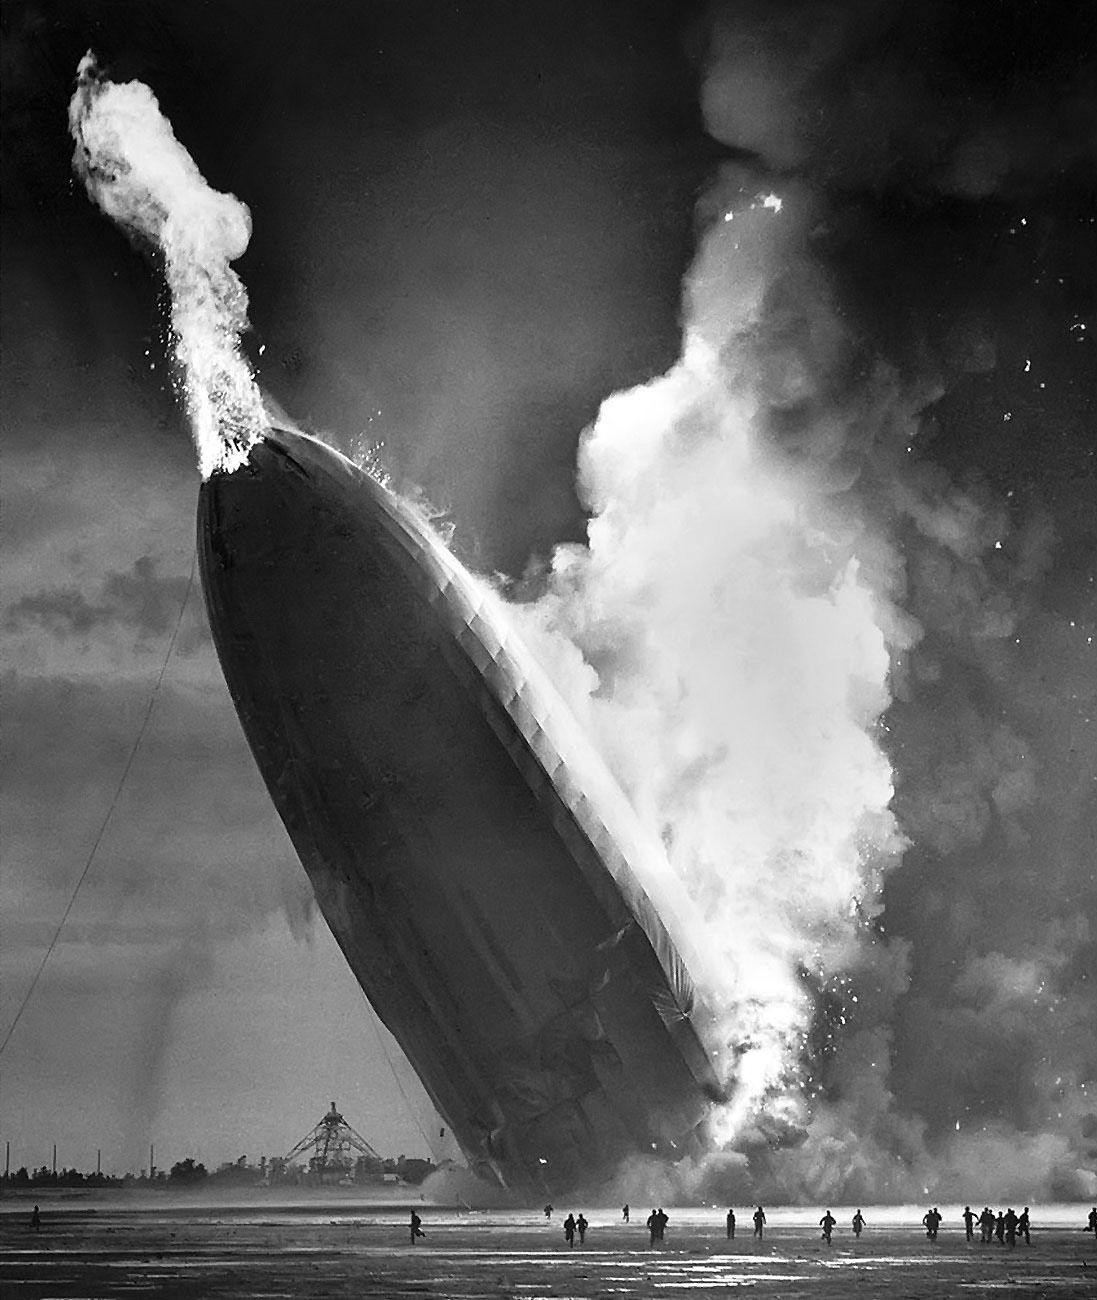
\includegraphics[height=0.9\paperheight]{Hindenburg_disaster,_1937.jpg}
    \end{center}
\end{frame}

\end{document}
